% Created 2018-10-19 vie 20:19
% Intended LaTeX compiler: pdflatex
\documentclass[xcolor={usenames,svgnames,dvipsnames}]{beamer}
\usepackage[utf8]{inputenc}
\usepackage[T1]{fontenc}
\usepackage{graphicx}
\usepackage{grffile}
\usepackage{longtable}
\usepackage{wrapfig}
\usepackage{rotating}
\usepackage[normalem]{ulem}
\usepackage{amsmath}
\usepackage{textcomp}
\usepackage{amssymb}
\usepackage{capt-of}
\usepackage{hyperref}
\usepackage{color}
\usepackage{listings}
\usepackage{mathpazo}
\usepackage{gensymb}
\usepackage{amsmath}
\usepackage{chemarr}%flechas para reacciones químicas (SFER.tex)
\bibliographystyle{plain}
\AtBeginSubsection[]{\begin{frame}[plain]\tableofcontents[currentsubsection,sectionstyle=show/shaded,subsectionstyle=show/shaded/hide]\end{frame}}
\AtBeginSection[]{\begin{frame}[plain]\tableofcontents[currentsection,hideallsubsections]\end{frame}}
\usepackage[emulate=units]{siunitx}
\sisetup{fraction=nice, decimalsymbol=comma, retain-unity-mantissa = false}
\newunit{\wattpeak}{Wp}
\newunit{\watthour}{Wh}
\newunit{\amperehour}{Ah}
\usepackage{steinmetz}
\hypersetup{colorlinks=true, linkcolor=Blue, urlcolor=Blue}
\renewcommand{\thefootnote}{\fnsymbol{footnote}}
\beamertemplatenavigationsymbolsempty
\setbeamertemplate{footline}[frame number]
\setbeamercolor{alerted text}{fg=blue!50!black} \setbeamerfont{alerted text}{series=\bfseries}
\usetheme[hideothersubsections]{Goettingen}
\usecolortheme{rose}
\usefonttheme{serif}
\author{Oscar Perpiñán Lamigueiro}
\date{\url{http://oscarperpinan.github.io}}
\title{Electrotecnia}
\hypersetup{
 pdfauthor={Oscar Perpiñán Lamigueiro},
 pdftitle={Electrotecnia},
 pdfkeywords={},
 pdfsubject={},
 pdfcreator={Emacs 25.2.2 (Org mode 9.1.13)}, 
 pdflang={Spanish}}
\begin{document}

\maketitle

\section{Conceptos preliminares}
\label{sec:org4c46145}

\begin{frame}[label={sec:orgfcef17e}]{Electricidad}
\begin{itemize}
\item La electricidad es un fenómeno físico asociado al \alert{movimiento de las
cargas eléctricas}.

\item El aprovechamiento de la electricidad consiste en generar y canalizar
el movimiento de las cargas eléctricas.

\item El movimiento de las cargas eléctricas es la \alert{corriente eléctrica}.
Este movimiento se realiza mediante un trabajo, cuantificado por el
\alert{potencial}.
\end{itemize}
\end{frame}

\begin{frame}[label={sec:org95ba2cf}]{Intensidad de Corriente eléctrica}
\begin{itemize}
\item \alert{Variación de la carga con el tiempo en la sección transversal de un
conductor} \(i(t)=\frac{dq(t)}{dt}\)

\item Movimiento de electrones libres. Sin embargo, por convenio su sentido
es positivo para el movimiento de las cargas positivas.
\end{itemize}
\end{frame}

\begin{frame}[label={sec:org7ecbc50}]{Principio de conservación de la carga}
\begin{itemize}
\item Las lineas de corriente son cerradas (o solenoidales)

\item \alert{Ley de Kirchhoff de las corrientes (LKC)}: la suma de las corrientes
que llegan a un nudo es igual a la suma de las que salen.
\end{itemize}

\begin{center}
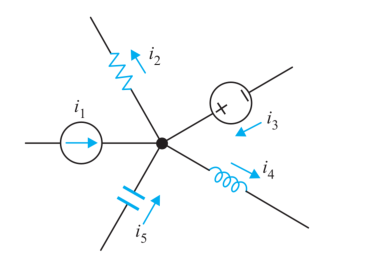
\includegraphics[height=0.5\textheight]{/home/oscar/github/esf/figs/LKC_FM.pdf}
\end{center}

\[
i_1(t) - i_2(t) + i_3(t) - i_4(t) + i_5(t) = 0
\]
\end{frame}

\begin{frame}[label={sec:orgbee1557}]{Tensión. Diferencia de potencial}
\begin{itemize}
\item \alert{Trabajo realizado al mover una carga unidad entre dos puntos}.
\end{itemize}

\[
v=\frac{dW_{e}}{dq}
\]

\begin{itemize}
\item Si entre dos puntos A y B existe una diferencia de potencial, podemos
escribir:
\end{itemize}
\begin{align*}
         v_{AB} &=  v_{A}-v_{B}\\
         v_{AB} &=  -v_{BA}
\end{align*}
\end{frame}

\begin{frame}[label={sec:orgc7427bc}]{Principio de conservación de la energía}
\begin{itemize}
\item La energía producida por un generador se consume por los receptores
del circuito para producir trabajo (mecánico, químico, etc.) o
calor.

\item \alert{Ley de Kirchhoff de los Voltajes (LKV)}: la suma (con signo) de las
tensiones a lo largo de un camino cerrado (circuito) es cero.
\end{itemize}

\begin{center}
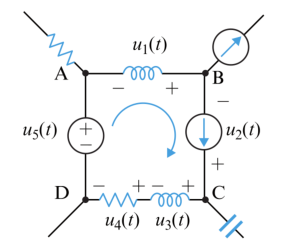
\includegraphics[height=0.5\textheight]{/home/oscar/github/esf/figs/LKV_FM.pdf}
\end{center}

\[
u_3(t) + u_4 (t) - u_5 (t) - u_1 (t) - u_2 (t)  = 0
\]
\end{frame}

\begin{frame}[label={sec:org577f4b7}]{Potencia eléctrica}
\begin{itemize}
\item Trabajo realizado por unidad de tiempo
\end{itemize}
\[
p(t)=\frac{dW_{e}}{dt}=v(t)\cdot\frac{dq(t)}{dt}=v(t)\cdot i(t)
\]

\begin{itemize}
\item Un elemento del circuito absorbe (\emph{receptor}) o entrega
(\emph{generador}) potencia según el sentido de tensión y corriente en
sus terminales. Ejemplo: en el dipolo de la figura se absorbe
potencia (\(p(t)>0\))
\end{itemize}
\begin{center}
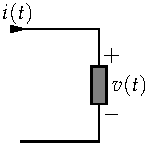
\includegraphics[height=0.5\textheight]{../figs/ReceptorPasivo.pdf}
\end{center}
\end{frame}

\begin{frame}[label={sec:orga6d284f}]{Potencia y Energía}
\begin{description}
\item[{Energía}] es la capacidad para realizar un trabajo.

Unidades Wh, kWh

1 kWh = 3.6 MJ

\item[{Potencia}] es la cantidad de trabajo efectuado \emph{por unidad de
tiempo}.

Unidades W, kW
\end{description}
\end{frame}

\begin{frame}[label={sec:org3c819f9}]{Eficiencia y Rendimiento}
\begin{description}
\item[{Eficiencia}] de un proceso es la relación entre la \emph{potencia} de
salida y la \emph{potencia} de entrada a ese proceso.

\item[{Rendimiento}] de un proceso es la relación entre la \emph{energía} de
salida y la \emph{energía} de entrada a ese proceso.
\end{description}
\end{frame}

\section{Elementos del Circuito}
\label{sec:orgf782fde}
\subsection{Elementos Lineales}
\label{sec:orgefa1ccd}

\begin{frame}[label={sec:org2f0533d}]{Generadores}
\begin{itemize}
\item \alert{Generador de tensión}: su tensión es independiente de la corriente
(la corriente la fija el circuito)

\begin{itemize}
\item Batería electroquímica

\item Inversor de electrificación rural a su salida
\end{itemize}
\end{itemize}
\begin{center}
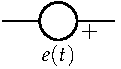
\includegraphics[height=0.2\textheight]{../figs/GeneradorTension.pdf}
\end{center}

\begin{itemize}
\item \alert{Generador de corriente}: su corriente es independiente de la tensión
(la tensión la fija el circuito)

\begin{itemize}
\item Inversor de conexión a red a su salida
\end{itemize}
\end{itemize}
\begin{center}
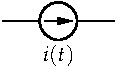
\includegraphics[height=0.2\textheight]{../figs/GeneradorCorriente.pdf}
\end{center}
\end{frame}

\begin{frame}[label={sec:orgef25b63}]{Resistencia}
\begin{center}
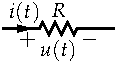
\includegraphics[height=0.2\textheight]{../figs/Resistencia.pdf}
\end{center}


\begin{itemize}
\item \alert{Produce una caída de tensión entre sus terminales directamente
proporcional a la corriente que lo atraviesa}.
\end{itemize}
\[
V=R\cdot I
\]
\begin{itemize}
\item La constante de proporcionalidad es el valor de la resistencia

\item Su valor depende de resistividad del material, de la sección y de la
longitud: \(R=\rho\cdot\frac{L}{S}\)
\end{itemize}
\end{frame}

\begin{frame}[label={sec:org3bd2c6f}]{Resistencia}
\begin{center}
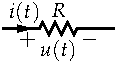
\includegraphics[height=0.2\textheight]{../figs/Resistencia.pdf}
\end{center}


\begin{itemize}
\item Disipa energía eléctrica produciendo \alert{calor}:
\end{itemize}
\[
p(t)=R\cdot i^{2}(t)
\]

\begin{itemize}
\item Cortocircuito: resistencia nula (tensión nula)

\item Circuito abierto: resistencia infinita (corriente nula).
\end{itemize}
\end{frame}


\begin{frame}[label={sec:org0dc51ad}]{Bobina o inductancia}
\begin{center}
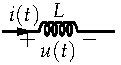
\includegraphics[height=0.2\textheight]{../figs/Bobina.pdf}
\end{center}


\begin{itemize}
\item Cuando una corriente oscilante atraviesa un conductor arrollado se
produce una \alert{tensión inducida que se opone a esta corriente} (ley de
Faraday y Lenz)

\item La constante que liga la tensión en sus terminales con el cambio de
la corriente es el valor de la inductancia
\end{itemize}

\[
v(t)=L\cdot\frac{di(t)}{dt}
\]
\end{frame}

\begin{frame}[label={sec:org547bbf2}]{Bobina o inductancia}
\begin{center}
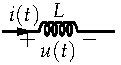
\includegraphics[height=0.2\textheight]{../figs/Bobina.pdf}
\end{center}


\begin{itemize}
\item Almacena \alert{energía magnética}.

\item La bobina \alert{retrasa los cambios de la corriente} respecto de la
tensión.

\item En circuitos de corriente continua es un cortocircuito.
\end{itemize}
\end{frame}

\begin{frame}[label={sec:org43aab33}]{Condensador}
\begin{center}
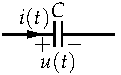
\includegraphics[height=0.2\textheight]{../figs/Condensador.pdf}
\end{center}

\begin{itemize}
\item \alert{Condensador}: dos placas metálicas separadas por una capa dieléctrica.

\item Al aplicar tensión se produce una \alert{separación de cargas opuestas que
se acumulan en cada placa}.

\item \alert{Capacidad}: constante de proporcionalidad entre carga y tensión.
\end{itemize}
\[
q(t) = C \cdot u(t)
\]

\begin{itemize}
\item En el proceso de carga se produce una corriente eléctrica entre las
dos placas.
\end{itemize}
\[
i(t)=\frac{dq(t)}{d(t)}=C\frac{du(t)}{dt}
\]
\end{frame}


\begin{frame}[label={sec:org94882b3}]{Condensador}
\begin{center}
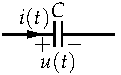
\includegraphics[height=0.2\textheight]{../figs/Condensador.pdf}
\end{center}

\begin{itemize}
\item Almacena \alert{energía eléctrica}

\item \alert{Retrasa las variaciones de la tensión respecto de la corriente}

\item En un circuito de corriente continua se comporta como un circuito
abierto.
\end{itemize}
\end{frame}

\subsection{Elementos No Lineales}
\label{sec:orgafa730a}

\begin{frame}[label={sec:org8cf424f}]{Diodo}
\begin{center}
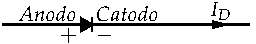
\includegraphics[height=0.15\textheight]{../figs/Diodo.pdf}
\end{center}

\begin{itemize}
\item Un diodo es un dispositivo electrónico que permite el paso de
corriente a través de él a partir de una tensión de polarización.

\item Cuando \alert{no conduce} se comporta (idealmente) como un \alert{circuito abierto}.

\item Cuando \alert{conduce} se comporta (idealmente) como un \alert{cortocircuito}.
\end{itemize}
\end{frame}

\begin{frame}[label={sec:orgfec8928}]{Diodo}
\begin{center}
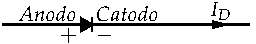
\includegraphics[height=0.15\textheight]{../figs/Diodo.pdf}
\end{center}

\begin{itemize}
\item Por tanto, puede ser utilizado como

\begin{itemize}
\item \alert{Elemento de bloqueo} (evitar que circule corriente por una parte
del circuito en ciertas condiciones)

\item \alert{Elemento de protección} (obligar a que la corriente circule por
él, evitando que circule por otra rama paralela).
\end{itemize}
\end{itemize}
\end{frame}

\begin{frame}[label={sec:org3e12b06}]{Transistor}
\begin{center}
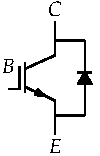
\includegraphics[height=0.3\textheight]{../figs/Transistor.pdf}
\end{center}

\begin{itemize}
\item Un transistor es un dispositivo electrónico con tres terminales que
permite el paso de corriente entre dos de sus terminales cuando en el
tercer terminal está polarizado adecuadamente.

\item Cuando \alert{no conduce} se comporta (idealmente) como un \alert{circuito abierto}.

\item Cuando \alert{conduce} se comporta (idealmente) como un \alert{cortocircuito}.
\end{itemize}
\end{frame}


\begin{frame}[label={sec:org5c0b312}]{Transistor}
\begin{center}
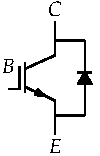
\includegraphics[height=0.3\textheight]{../figs/Transistor.pdf}
\end{center}

Por tanto, puede ser utilizado como:

\begin{itemize}
\item \alert{Elemento de conmutación} (dirigir la circulación de corriente entre
dos terminales controlando la señal en el tercer terminal)

\item \alert{Elemento de amplificación} (la señal entregada en el terminal de
control es reproducida en la salida con mayor amplitud)
\end{itemize}
\end{frame}

\subsection{Asociación de elementos pasivos}
\label{sec:org595dcf8}

\begin{frame}[label={sec:org29c6177}]{Conexión en serie}
\begin{block}{Misma corriente por todos los elementos: la tensión se reparte}
\(R_{s}=\sum_{i}R_{i}\)

\(L_{s}=\sum_{i}L_{i}\)

\(\frac{1}{C_{s}}=\sum_{i}\frac{1}{C_{i}}\)
\begin{center}
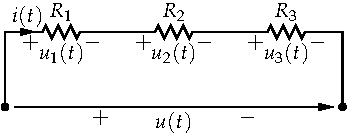
\includegraphics[height=0.3\textheight]{../figs/AsociacionSerie.pdf}
\end{center}
\end{block}
\end{frame}

\begin{frame}[label={sec:org72dfe85}]{Conexión en paralelo}
\begin{block}{Misma tensión aplicada a todos los elementos: la corriente se reparte}
\(\frac{1}{R_{p}}=\sum_{i}\frac{1}{R_{i}}\)

\(\frac{1}{L_{p}}=\sum_{i}\frac{1}{L_{i}}\)

\(C_{p}=\sum_{i}C_{i}\)
\begin{center}
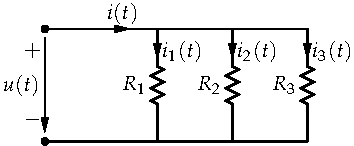
\includegraphics[height=0.3\textheight]{../figs/AsociacionParalelo.pdf}
\end{center}
\end{block}
\end{frame}


\section{Corriente alterna sinusoidal}
\label{sec:orga54e95a}

\subsection{Conceptos Fundamentales}
\label{sec:orgd3e5897}

\begin{frame}[label={sec:orgd2f6ee5}]{Onda sinusoidal}
\begin{center}
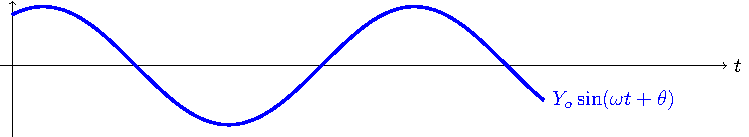
\includegraphics[width=.9\linewidth]{../figs/sin.pdf}
\end{center}


\[
y(t)=Y_{o}\cdot\sin(\omega\cdot t+\theta)
\]

\begin{itemize}
\item \(Y_{o}\) valor máximo de la onda.

\item \(\omega=\frac{2\cdot\pi}{T}\): pulsación (radianes/segundo)

\item T: periodo de la onda (segundos)

\item \(f=\frac{\omega}{2\cdot\pi}=\frac{1}{T}\): frecuencia (Hz)
\end{itemize}
\end{frame}


\begin{frame}[label={sec:orgd709414}]{Fase}
\begin{center}
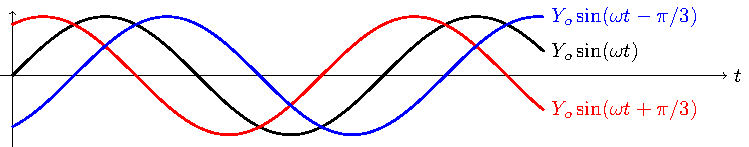
\includegraphics[width=.9\linewidth]{../figs/desfase.pdf}
\end{center}


\[
y(t)=Y_{o}\cdot\sin(\omega\cdot t+\theta)
\]

\begin{itemize}
\item \(\theta\): fase (radianes o grados)

\begin{itemize}
\item Es el argumento de la onda para t=0

\item Tomando una onda como referencia, si la fase es 0º, se dice que
están en fase con la onda de referencia.

\item Si la fase es positiva, se dice que la onda adelanta
respecto a la referencia.
\end{itemize}
\end{itemize}
\end{frame}


\begin{frame}[label={sec:org3a5af42}]{Señales en Cuadratura}
\begin{center}
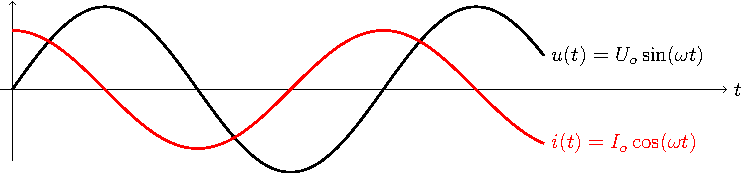
\includegraphics[width=.9\linewidth]{../figs/cuadratura.pdf}
\end{center}

\begin{itemize}
\item Cuando el desfase entre dos señales es de 90º (\(\theta_I - \theta_U = \pi/2\)), se dice que están en cuadratura.
\item El paso por cero de una señal coincide con el paso por el máximo/mínimo de la otra señal.
\end{itemize}
\end{frame}


\begin{frame}[label={sec:orga693648}]{Valor medio y valor eficaz}
\begin{block}{Valor medio}
\[
Y_m=\frac{1}{T}\int_{0}^{T}y(t)
\]

\[
Y_m=\frac{1}{T}\int_{0}^{T}Y_{o}\cdot\sin(\omega\cdot+\theta)\, dt=0
\]
\end{block}
\begin{block}{Valor eficaz}
\[
Y = \sqrt{\frac{1}{T}\cdot\int_{0}^{T}y^{2}(t)}
\]

\[
Y=\sqrt{\frac{1}{T}\cdot\int_{0}^{T}\left(Y_{o}\cdot\sin(\omega\cdot t+\theta)\right)^{2}dt}=\frac{Y_{o}}{\sqrt{2}}
\]
\end{block}
\end{frame}
\subsection{Cálculo Fasorial}
\label{sec:org66ff445}

\begin{frame}[label={sec:org1eaaf2a}]{Representación fasorial}
\begin{itemize}
\item Un fasor es un \alert{número complejo} que representa una señal sinusoidal para simplificar cálculos.
\item El \alert{módulo} del fasor es el \alert{valor eficaz}. El \alert{argumento} es la \alert{fase}.
\item Descartamos pulsación: No se puede emplear cuando hay frecuencias diferentes en un mismo circuito.
\end{itemize}

\begin{columns}
\begin{column}{0.5\columnwidth}
\begin{align*}
\overline{Y} &= Y\cdot e^{j\theta}\\
\overline{Y} &= Y\cdot(\cos(\theta)+\mathrm{j}\cdot\sin(\theta))\\
\overline{Y} &= Y\phase{\theta}
\end{align*}
\end{column}

\begin{column}{0.5\columnwidth}
\begin{center}
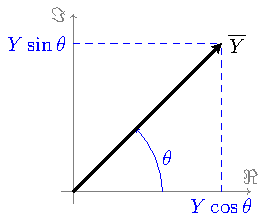
\includegraphics[height=0.45\textheight]{../figs/fasor.pdf}
\end{center}
\end{column}
\end{columns}
\end{frame}


\begin{frame}[label={sec:org3d3542c}]{Impedancia}
\begin{columns}
\begin{column}{0.4\columnwidth}
\begin{align*}
  \overline{I} &= I\phase{\theta_I}\\
  \overline{U} &= U\phase{\theta_U}
\end{align*}

\begin{align*}
  \overline{U} &= \overline{Z} \cdot \overline{I}\\                 
  \overline{Z} &= \frac{\overline{U}}{\overline{I}}
\end{align*}

\[
\overline{Z} = \frac{U}{I}\phase{\theta_U - \theta_I} = 
    \begin{cases}
      Z = \frac{U}{I}\\
      \theta_Z = \theta_U - \theta_I
    \end{cases}
\]
\end{column}

\begin{column}{0.6\columnwidth}
\begin{center}
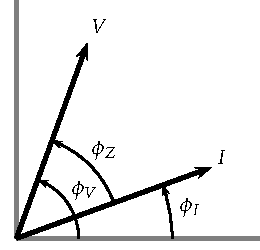
\includegraphics[height=0.5\textheight]{../figs/Impedancia.pdf}
\end{center}
\end{column}
\end{columns}
\end{frame}

\begin{frame}[label={sec:orgb1996ca}]{Impedancia de los Elementos: Resistencia}
\[
\overline{Z}_R = R = R\phase{0}
\]

\begin{center}
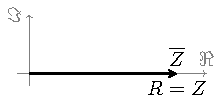
\includegraphics[width=.9\linewidth]{../figs/fasorResistencia.pdf}
\end{center}
\end{frame}

\begin{frame}[label={sec:orgf861eb1}]{Impedancia de los Elementos: Inductancia}
\begin{columns}
\begin{column}{0.4\columnwidth}
\[
\overline{Z}_L = j\omega L = \omega L \phase{\ang{90}} \Rightarrow X_L = \omega L
\]
\end{column}

\begin{column}{0.6\columnwidth}
\begin{center}
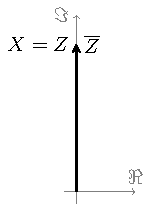
\includegraphics[width=.9\linewidth]{../figs/fasorInductancia.pdf}
\end{center}
\end{column}
\end{columns}
\end{frame}

\begin{frame}[label={sec:org4c5ef10}]{Impedancia de los Elementos: Condensador}
\begin{columns}
\begin{column}{0.4\columnwidth}
\[
\overline{Z}_C = \frac{1}{j\omega C} = \frac{1}{\omega C}\phase{\ang{-90}} \Rightarrow X_C = \frac{1}{\omega C}
\]
\end{column}
\begin{column}{0.6\columnwidth}
\begin{center}
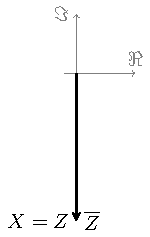
\includegraphics[width=.9\linewidth]{../figs/fasorCondensador.pdf}
\end{center}
\end{column}
\end{columns}
\end{frame}

\begin{frame}[label={sec:orga9eb4ec}]{Impedancia Genérica}
\[
\overline{Z} = R + j X
\]

\begin{center}
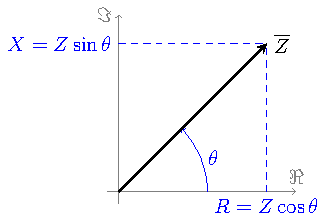
\includegraphics[width=.9\linewidth]{../figs/fasorImpedancia.pdf}
\end{center}
\end{frame}

\subsection{Desfase Tensión - Corriente}
\label{sec:org195ad6f}
\begin{frame}[label={sec:org728b45f}]{Convenio de signos para Desfase}
\begin{itemize}
\item En general, la tensión es origen de fases (\(\theta_{V}=0\)).
\end{itemize}
\begin{align*}
\theta_Z &= \theta_U - \theta_I\\
\theta_{I} &= \theta_{V}- \theta_{Z} = -\theta
\end{align*}

\begin{itemize}
\item La corriente está retrasada respecto de la tensión un ángulo \(\theta = \theta_Z\):
\end{itemize}
\begin{align*}
  u(t) &= U_{o}\cdot\sin(\omega \cdot t)\\
  i(t) &= I_{o}\cdot\sin(\omega \cdot t - \theta)
\end{align*}
\end{frame}

\begin{frame}[label={sec:orgfd21745}]{Circuito Resistivo}
\[
\overline{Z}_R = R = R \phase{0}
\]

\begin{center}
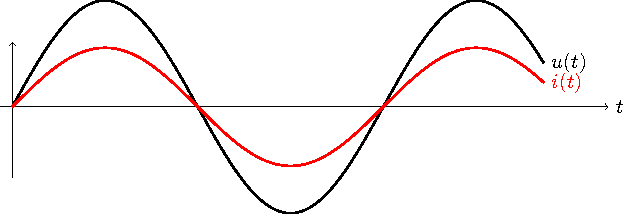
\includegraphics[width=.9\linewidth]{../figs/resistivo.pdf}
\end{center}

Un circuito resistivo no desfasa (\alert{tensión y corriente en fase}).
\end{frame}

\begin{frame}[label={sec:org233a2ab}]{Circuito Inductivo puro}
\[
\overline{Z}_L = j\omega L = \omega L \phase{\ang{90}}
\]

\begin{center}
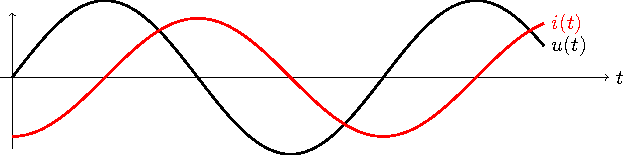
\includegraphics[width=.9\linewidth]{../figs/inductivoPuro.pdf}
\end{center}

Un circuito inductivo puro genera \alert{señales en cuadratura} y \alert{retrasa la corriente}.
\end{frame}

\begin{frame}[label={sec:org2f016b5}]{Circuito Capacitivo puro}
\[
\overline{Z}_C = \frac{1}{j\omega C} = \frac{1}{\omega C}\phase{\ang{-90}}
\]

\begin{center}
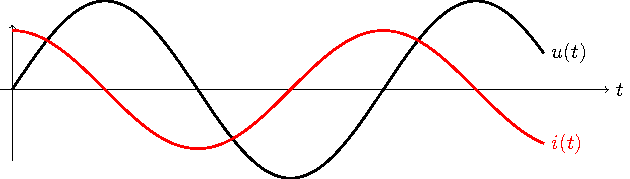
\includegraphics[width=.9\linewidth]{../figs/capacitivoPuro.pdf}
\end{center}


Un circuito capacitivo puro genera \alert{señales en cuadratura} y \alert{adelanta la corriente}.
\end{frame}

\begin{frame}[label={sec:org21ad8c7}]{Circuito Inductivo con pérdidas}
\[
\overline{Z} = R + j\omega L \Rightarrow \theta > 0
\]

\begin{center}
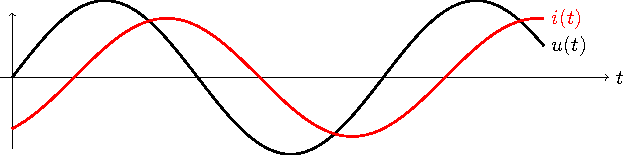
\includegraphics[width=.9\linewidth]{../figs/inductivo.pdf}
\end{center}

Un circuito inductivo \alert{retrasa la corriente}.
\end{frame}

\begin{frame}[label={sec:orgdbe384b}]{Circuito Capacitivo con pérdidas}
\[
\overline{Z} = R - \frac{j}{\omega C} \Rightarrow \theta < 0
\]

\begin{center}
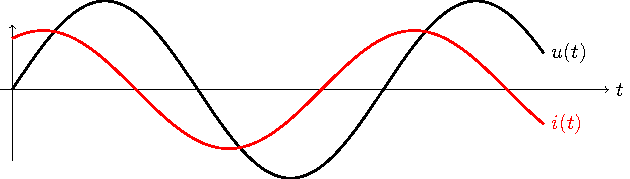
\includegraphics[width=.9\linewidth]{../figs/capacitivo.pdf}
\end{center}

Un circuito capacitivo \alert{adelanta la corriente}.
\end{frame}

\subsection{Potencia}
\label{sec:org58f09e6}

\begin{frame}[label={sec:orgd53c9fd}]{Circuito Resistivo}
\begin{center}
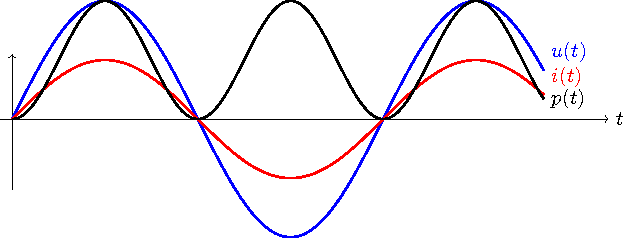
\includegraphics[width=.9\linewidth]{../figs/resistivoPotencia.pdf}
\end{center}

\begin{itemize}
\item Fluctúa al doble de frecuencia.
\item Es siempre positiva.
\end{itemize}
\[
  p(t) = R i^2(t) = \frac{u^2(t)}{R}
\]
\end{frame}
\begin{frame}[label={sec:org3a8027c}]{Circuito Inductivo puro}
\begin{center}
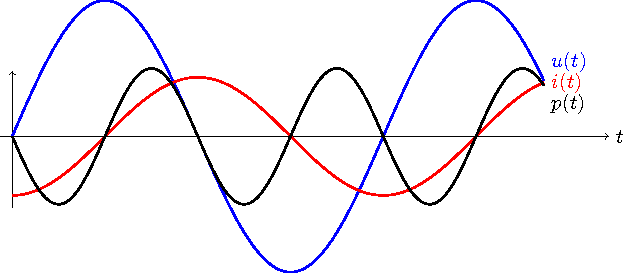
\includegraphics[width=.9\linewidth]{../figs/inductivoPuroPotencia.pdf}
\end{center}

\begin{itemize}
\item Fluctúa al doble de frecuencia.
\item Pasa por los ceros de tensión y corriente.
\item Su valor medio es nulo.
\end{itemize}
\end{frame}


\begin{frame}[label={sec:org39b336e}]{Circuito Capacitivo puro}
\begin{center}
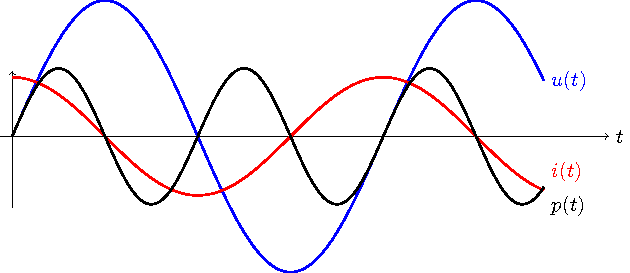
\includegraphics[width=.9\linewidth]{../figs/capacitivoPuroPotencia.pdf}
\end{center}

\begin{itemize}
\item Fluctúa al doble de frecuencia.
\item Pasa por los ceros de tensión y corriente.
\item Su valor medio es nulo.
\end{itemize}
\end{frame}

\begin{frame}[label={sec:org36ed404}]{Circuito Inductivo con pérdidas}
\begin{center}
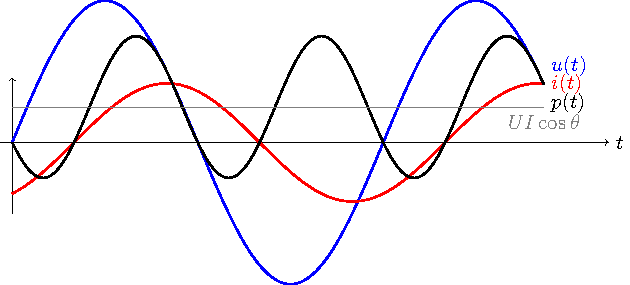
\includegraphics[width=.9\linewidth]{../figs/inductivoPotencia.pdf}
\end{center}

\begin{itemize}
\item Su valor medio es positivo, de valor \(U I \cos \theta\).
\end{itemize}
\end{frame}

\begin{frame}[label={sec:org8aa114c}]{Circuito Capacitivo con pérdidas}
\begin{center}
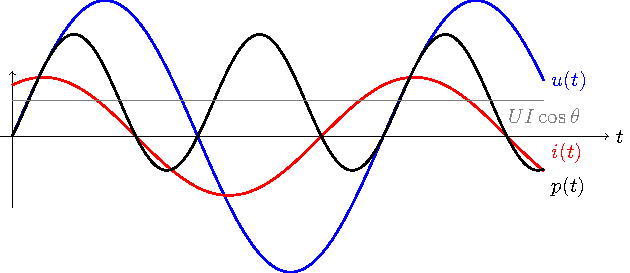
\includegraphics[width=.9\linewidth]{../figs/capacitivoPotencia.pdf}
\end{center}

\begin{itemize}
\item Su valor medio es positivo, de valor \(U I \cos \theta\).
\end{itemize}
\end{frame}

\begin{frame}[label={sec:org9e93ed1}]{Triángulo de Potencias}
\begin{columns}
\begin{column}{0.4\columnwidth}
\begin{itemize}
\item Potencia Activa
\end{itemize}
\[  
P = U\cdot I\cdot\cos(\theta) = R \cdot I^2
\]

\begin{itemize}
\item Potencia Reactiva
\end{itemize}
\[
Q = U\cdot I\cdot\sin(\theta) = X \cdot I^2
\]

\begin{itemize}
\item Potencia Aparente
\end{itemize}
\[
\overline{S} = P + jQ = \overline{U} \cdot \overline{I}^*
\]
\[
|S| = U \cdot I
\]
\[
\theta_S = \theta_Z = \theta
\]
\end{column}

\begin{column}{0.6\columnwidth}
\begin{center}
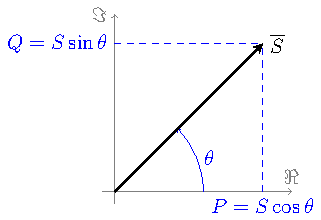
\includegraphics[width=.9\linewidth]{/home/oscar/github/esf/figs/trianguloPotencias.pdf}
\end{center}
\end{column}
\end{columns}
\end{frame}

\begin{frame}[label={sec:org1211e79}]{Potencia de elementos: Resistencia}
\[
\theta = 0 \Rightarrow 
\begin{cases}
  P_R = R I^2\\
  Q_R = 0\\
  S_R = P_R
\end{cases}
\]

\begin{itemize}
\item Consume potencia activa
\item No consume potencia reactiva
\end{itemize}
\end{frame}

\begin{frame}[label={sec:org4bbc627}]{Potencia de elementos: Inductancia}
\[
\theta = \pi/2 \Rightarrow 
\begin{cases}
  P_L = 0\\
  Q_L = \omega L I^2\\
  \overline{S}_L = \omega L I^2 \phase{\pi/2}
\end{cases}
\]

\begin{itemize}
\item No consume potencia activa
\item Consume potencia reactiva (\(Q > 0\))
\end{itemize}
\end{frame}

\begin{frame}[label={sec:orgb4a9dc4}]{Potencia de elementos: Condensador}
\[
\theta = - \pi/2 \Rightarrow 
\begin{cases}
  P_L = 0\\
  Q_C = - \omega C U^2\\
  \overline{S}_C = \omega C U^2 \phase{-\pi/2}
\end{cases}
\]

\begin{itemize}
\item No consume potencia activa
\item Genera potencia reactiva (\(Q < 0\))
\end{itemize}
\end{frame}

\begin{frame}[label={sec:org1230bd3}]{Teorema de Boucherot}
\begin{itemize}
\item En un circuito con múltiples elementos, la potencia aparente total es la suma de las potencias aparentes individuales.
\end{itemize}
\begin{align*}
  \overline{S} &= \sum_{i = 1}^{n} S_i\\
  P + jQ &= \sum^n_{i = 1} (P_i + jQ_i)
\end{align*}

\begin{itemize}
\item La potencia activa (reactiva) total es la suma de las potencias activas (reactivas) individuales.
\end{itemize}

\begin{align*}
P &= \sum_{i = 1}^n P_i\\
Q &= \sum_{i = 1}^n Q_i
\end{align*}
\end{frame}

\begin{frame}[label={sec:orgd7cb2c0}]{Compensación de reactiva}
\begin{itemize}
\item El factor de potencia, \(\cos(\theta)\), representa la aportación de potencia activa dentro de la potencia aparente.
\end{itemize}
\[
P = S \cos \theta
\]

\begin{itemize}
\item Sean dos sistemas con misma tensión y potencia activa, y factores de potencia \(\cos \theta_1 > \cos \theta_2\).

\item El sistema 2 requiere \alert{mayor sección} de cable para transportar la misma potencia activa.
\end{itemize}
\[
  \left(\frac{P}{U \cos \theta_1} = I_1 \right) < \left( I_2 = \frac{P}{U \cos \theta_2}\right) 
\]
\begin{itemize}
\item El sistema 2 requiere \alert{mayor potencia aparente} (generador mayor) para alimentar la misma potencia activa.
\end{itemize}
\[
  \left(\frac{P}{\cos \theta_1} = S_1 \right) < \left( S_2 = \frac{P}{\cos \theta_2}\right) 
\]
\end{frame}

\begin{frame}[label={sec:org30e5824}]{Compensación de reactiva}
\begin{itemize}
\item Comúnmente, el factor de potencia es \alert{inductivo} (máquinas eléctricas
industriales).

\item La red debe suministrar potencia reactiva inductiva (influye en secciones de líneas y tamaños de generadores)

\item Es necesario mejorar \alert{localmente} el factor de potencia. Solución
común: utilizar \alert{bancos de condensadores} como suministradores de
potencia reactiva.
\end{itemize}
\end{frame}

\begin{frame}[label={sec:org86b3523}]{Compensación de reactiva}
\begin{itemize}
\item Sea una carga de potencia activa \(P\) y potencia reactiva \(Q\). Supongamos que se desea mejorar el factor de potencia a \(\cos \theta' > \cos \theta\):
\end{itemize}

\[
  Q' = P \tan \theta'
\]

\[
  Q_c = Q - Q' = P \tan \theta - P \tan \theta'
\]

\[
  Q_c = \omega C U^2
\]

\[
C = \frac{P (\tan \theta - \tan \theta')}{\omega U^2}
\]
\end{frame}


\subsection{Trifásica}
\label{sec:org4692e3c}

\begin{frame}[label={sec:org49e3fab}]{Motivación de los sistemas trifásicos}
\begin{itemize}
\item La potencia instantánea de un sistema monofásico es pulsante. En un
sistema trifásico la potencia instantánea es constante, evitando
vibraciones y esfuerzos en las máquinas.

\item Para transportar una determinada potencia la masa de conductor
necesaria es un 25\% en un trifásico que en un monofásico.
\end{itemize}
\end{frame}

\begin{frame}[label={sec:orgd6594c9}]{Generación de un sistema trifásico}
\begin{center}
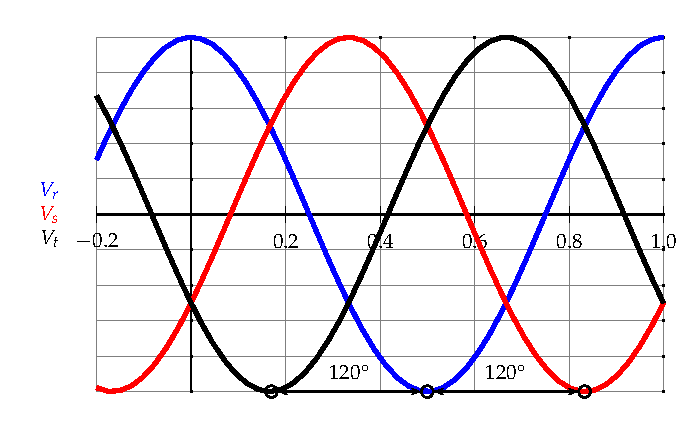
\includegraphics[width=.9\linewidth]{../figs/TensionesTrifasica.pdf}
\end{center}
\end{frame}

\begin{frame}[label={sec:org798b9e3}]{Receptores}
\begin{itemize}
\item \alert{Tensión simple o de fase}: la existente entre una fase y el neutro.
\item \alert{Tensión compuesta o de línea} (por defecto): la existente entre dos fases.
\item Un receptor puede estar conectado en \alert{estrella} (punto común) o en \alert{triángulo}.
\item Un receptor puede ser \alert{equilibrado} (las tres impedancias que lo componen son idénticas) o \alert{desequilibrado}.
\item Cuando el receptor es equilibrado la corriente que circula por el neutro es nula.
\end{itemize}
\end{frame}

\begin{frame}[label={sec:org150d2da}]{Fase y línea}
\begin{block}{Receptor en Estrella (cuatro hilos, 3F+1N)}
\(V_{L}=\sqrt{3}\cdot V_{F}\) 

\(I_{F}=I_{L}\)

\(P=3\cdot V_{F}I_{F}\cos(\theta)=\sqrt{3}V_{L}I_{L}\cos(\theta)\)
\begin{center}
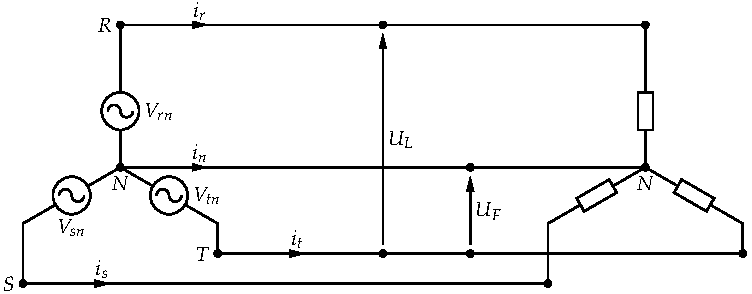
\includegraphics[width=.9\linewidth]{../figs/RedTrifasicaEstrella.pdf}
\end{center}
\end{block}
\end{frame}

\begin{frame}[label={sec:org1a2dda4}]{Fase y línea}
\begin{block}{Receptor en Estrella (cuatro hilos, 3F+1N)}
\(V_{L}=\sqrt{3}\cdot V_{F}\) 

\(I_{F}=I_{L}\)

\(P=3\cdot V_{F}I_{F}\cos(\theta)=\sqrt{3}V_{L}I_{L}\cos(\theta)\)
\begin{center}
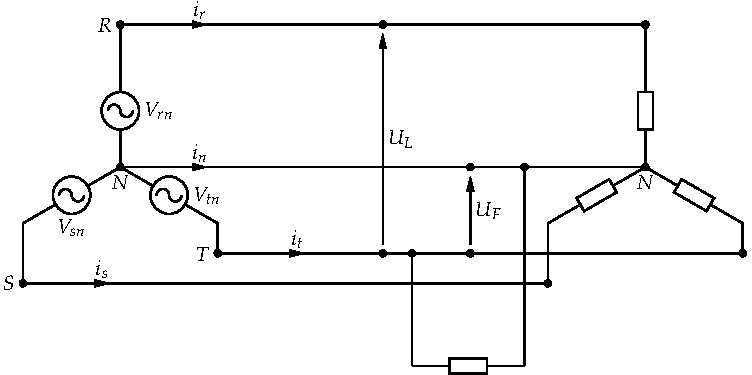
\includegraphics[width=.9\linewidth]{../figs/RedTrifasicaEstrella_CargaMonofasica.pdf}
\end{center}
\end{block}
\end{frame}

\begin{frame}[label={sec:org2d149f6}]{Fase y línea}
\begin{block}{Receptor en Triangulo (tres hilos, 3F)}
\(V_{L}=V_{F}\) 

\(I_{F}=\frac{I_{L}}{\sqrt{3}}\)

\(P=3\cdot V_{F}\cdot I_{F}\cos(\theta)=\sqrt{3}V_{L}I_{L}\cos(\theta)\)
\begin{center}
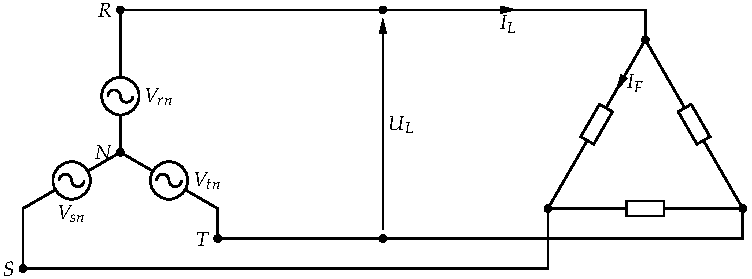
\includegraphics[width=.9\linewidth]{../figs/RedTrifasicaEstrella_CargaTriangulo.pdf}
\end{center}
\end{block}
\end{frame}

\begin{frame}[label={sec:orga9cdc11}]{Compensación de Reactiva}
Para mejorar el factor de potencia en un sistema trifásico equilibrado se deben emplear \alert{tres condensadores conectados en triángulo}:

\[
  C_\triangle = \frac{P(\tan \theta - \tan \theta')}{3\omega U^2}
\]
\end{frame}

\section{Recursos}
\label{sec:orgdb13210}

\begin{frame}[label={sec:org11c94df}]{Bibliografía}
\begin{itemize}
\item \alert{Fraile Mora, J.}: \emph{Circuitos Eléctricos}. Ed. Prentice Hall.

\item \alert{Hayt, W. y Kemmerly, J}: \emph{Análisis de circuitos en ingeniería}. Ed.
Mc. Graw Hill.

\item \alert{C. K. Alexander; M. N. O. Sadiku}, Ed. McGraw-Hill.

\item \href{http://tuveras.com/index.html}{Tú verás}
\end{itemize}
\end{frame}
\end{document}